\documentclass{article}

\usepackage{amsmath, amssymb}
\usepackage{float}
\usepackage{graphicx}
\usepackage{subcaption}
\usepackage{color}
\usepackage[table,xcdraw]{xcolor}

\usepackage{polski}

\usepackage{listings}


\definecolor{dkgreen}{rgb}{0,0.6,0}
\definecolor{gray}{rgb}{0.5,0.5,0.5}
\definecolor{mauve}{rgb}{0.58,0,0.82}

\lstset{frame=tb,
  language=C++,
  aboveskip=3mm,
  belowskip=3mm,
  showstringspaces=false,
  columns=flexible,
  basicstyle={\small\ttfamily},
  numberstyle=\color{gray},
  keywordstyle=\color{blue},
  commentstyle=\color{dkgreen},
  stringstyle=\color{mauve},
  breaklines=true,
  breakatwhitespace=true,
  tabsize=3,
}
%

\addtolength{\topmargin}{-.875in}
\addtolength{\textheight}{1.75in}


\begin{document}
\title{
\huge {Generator Krzywych Lissajous} \\
}

\author{Arkadiusz Trojanowski, Michał Żoczek, Wiktor Żychowicz}
\date{7 czerwca 2020}
\maketitle
\section{Założenia wstępne przyjęte w realizacji projektu}
	Program miał wyrysowywać odpowiednik krzywych Lissajous w trzech wymiarach. Użytkownik operując na dziewięciu suwakach reprezentujących wartości zmiennych$ A, B, C, \Theta, \Psi, \Phi$ oraz n, m k wpływał na kształt krzywej. Powinna istnieć możliwość rysowania obiektu we współrzędnych kartezjańskich, jak również biegunowych, w zależności od wyboru użytkownika. Program miał umożliwiać rysowanie kolorowych krzywych w formie oddzielnych punktów bądź też ciągłych linii zależnie od preferencji. Interfejs powinien również mieć zaimplementowaną możliwość obracania krzywych wokół trzech osi układu. Najbardziej atrakcyjną funkcją programu miała być możliwość animowania krzywych w formie dorysowywania kolejnych segmentów krzywej co dany krok czasowy, jak również płynnego zanikania końca krzywej, tak by na ekanie obserwować można było pojedynczą krzywą sunącą ustaloną wedle odpowiednich wzorów ścieżką.
	
\section{Specyfikacja danych wejściowych}
Krzywe Lissajous parametryzuje się wzorem:

\begin{equation}
	\left\{
                \begin{array}{ll}
                  x(t) = A \sin{nt + \Phi}\\
                  y(t) = B \sin{mt + \Psi}\\
                  z(t) = C \sin{kt + \Theta}
                \end{array}
              \right.
\end{equation}
lub dla współrzędnych sferycznych:
\begin{equation}
\left\{
                \begin{array}{ll}
                  r(t) = A \sin{nt + \Phi}\\
                  \alpha(t) = B \sin{mt + \Psi}\\
                  \beta(t) = C \sin{kt + \Theta}
                \end{array}
              \right.
\end{equation}
Dane wejściowe pobierane od użytkownika to rodzaj używanego układu współrzędnych, specyfikacja rysowania krzywych(linia, kropki) oraz możliwość zażądania animacji.
Narysowany obraz będzie można obrócić wzdłuż każdej osi za pomocą parametrów X, Y, Z. Jako jednostkę wartości kontowych postanowiono przyjąć stopnie.\\
Dodatkowo program ma dawać możliwość modyfikacji parametrów krzywych w odpowiednich zakresach:
\begin{itemize}
\item $A,B,C$ zakres [0,1]
\item $n, m, k$ zakres [0,10]
\item $\Theta, \Psi, \Phi, X , Y, Z$ zakres [0, 360]
\end{itemize}
 
\section{Oczekiwane dane wyjściowe}
Oczekiwanym rezultatem jest ciągła lub kropkowana krzywa narysowana w odpowiednim układzie współrzędnych oraz obrócona o odpowiednie kąty.\\
Dodatkową funkcjonalnością ma być animacja w formie blednącej na końcu serii kropek lub ciągłej linii biegnąca wzdłuż trasy wytyczonej przez wzory 1 lub 2. 
\section{Struktury danych}

		\subsection{Deque}
			Dwukierunkowa kolejka została użyta do przechowywania elementów krzywej w postaci segmentów.
			Zaimplementowana w postaci kontenera biblioteki standardowej C++ std::deque.
		\subsection{Color}
			\begin{lstlisting}
			struct Color
			{
			    Color(int _R, int _G, int _B) : R(_R), G(_G), B(_B) {}
			    Color next();
			    Color &operator+=(int i);
			
			    int R;
			    int G;
			    int B;
			private:
			    enum cycle
			    {
			        Ru,
			        Gu,
			        Rd,
			        Bu,
			        Gd,
			        Bd,
			    };
			    cycle current_cycle = Ru;
			    int m_step = 1;
			};
			\end{lstlisting}
			Struktura przechowująca kolor w postaci kodu RGB.\\
			Metoda \lstinline|next()| pozwala wygenerować następny kolor według schematu opisanego w sekcji Algorytmy.\\
			\lstinline|operator+=(int i)| służy do zwiększenia jasności koloru poprzez dodanie \lstinline|i| do każdego ze składników RGB.
		\subsection{Point}
			\begin{lstlisting}
				struct Point
				{
				    Point() = default;
				    Point(double x, double y, double z);
				    Point as_spherical();

				    double x = 0;
				    double y = 0;
				    double z = 0;
				};
			\end{lstlisting}
			Struktura przechowuje położenie punktu w postaci trzech współrzędnych w układzie kartezjańskim lub sferycznym.\\
			Metoda \lstinline|as_spherical()| pozwala na interpretację punktu zapisanego we współrzędnych sferycznych w układzie kartezjańskim (co jest konieczne aby poprawnie wyświetlić go na ekranie).
		\subsection{Segment}
			\begin{lstlisting}
				struct Segment
				{
				    Segment(Point _begin, Point _end, Color _color) : begin(_begin), end(_end), color(_color) {}
				
				    Point begin;
				    Point end;
				    Color color;
				};
			\end{lstlisting}
			Struktura przechowująca informacje dotyczące pojedynczego odcinka w postaci: punkt początkowy, punkt końcowy, kolor odcinka.
		\subsection{Vector4}
			\begin{lstlisting}
				struct Vector4
				{
				    friend Vector4 operator*(const Vector4&, double);
				
				    Vector4();
				    Vector4 operator-(const Vector4&);
				
				    void set(double d1, double d2, double d3);
				    double get_x();
				    double get_y();
				    double get_z();
				
				    double data[4];
				};
			\end{lstlisting}
			Struktura przechowująca wektor w postaci [x, y, z, t]. Podczas inicjalizacji t jest ustawiane na 1.\\
			\lstinline|operator*| pozwala wykonać mnożenie wektora przez skalar.
		\subsection{Matrix4}
			\begin{lstlisting}
				struct Matrix4
				{
				    friend Vector4 operator*(const Matrix4, const Vector4);
				
				    Matrix4();
				    Matrix4 operator*(const Matrix4);
				
				    double data[4][4];
				};
			\end{lstlisting}
			Struktura zawierająca macierz 4x4.\\
			Pozwala na operacje mnożenia wektorowego macierz $\times$ wektor i macierz $\times$ macierz.

\section{Interfejs użytkownika}
Do stworzenia interfejsu użytkownika użyto biblioteki wykorzystujące natywne kontrolki systemu. Interfejs składa się z panelu kontrolnego po lewej stronie okna oraz nieinteraktywny panelu przeznaczonego na rysownie krzywych. Wartości numeryczne można modyfikować za pomocą suwaków rozbudowanych o etykiety pokazujące aktualnie wybraną wartość. Wybór układu współrzędnych odbywa się przy pomocy dwóch przycisków u góry ekranu. Opcje rysowania i animacji użytkownik wybiera zaznaczając odpowiednie checkboxy, które same dbają, aby wybrane opcje ze sobą nie kolidowały poprzez automatyczne odznaczanie. 
\section{Wyodrębnienie i zdefiniowanie zadań}
Praca nad projektem została podzielona na dwie główne części: podstawową, na którą złożyły się implementacja GUI, utworzenie klas generujących odpowiednie segmenty krzywej na podstawie wartości ustawionych na suwakach, oraz właściwe rysowanie i obracanie krzywej na ekranie; oraz rozszerzoną, uwzględniającą wszelkie mniejsze poprawki i zaimplementowanie animacji.

\section{Użyta narzędzia programistyczne}
W projekcie zdecydowano użyć się biblioteki graficznej wxWidgets w celu skonstruowania GUI(dodatkowo skorzystano z programu wxFormBuilder) oraz użyto kilka funkcjonalności standardowej biblioteki C++(jedynego języka programowania użytego podczas tworzenia projektu). Każdy z programistów miał dowolność co do systemu operacyjnego, z którego mógł korzystać oraz użytego kompilatora. Jednak wszyscy zdecydowali pracować się na systemie Windows przy użyciu IDE Visual Studio. Praca była koordynowana przy pomocy sytemu kontroli wersji GIT poprzez użycie GitHuba. Dodatkowo komunikacja odbywała się za pomocą komunikatora głosowego Discord. 
\section{Podział pracy i analiza czasowa}
Prace nad projektem rozpoczęły się internetowym spotkaniem 15 maja i trwały trzy tygodnie, a każdy z nich kończył się kolejną konwersacją, na której wymieniane były spostrzeżenia i podporządkowywane były następne zadania. W pierwszym tygodniu wykonana została część podstawowa projektu:
\begin{itemize}
	\item zadaniem programisty Wiktora Żychowicza była implementacja interfejsu graficznego – stworzenie okna zawierającego wszelkie suwaki dla odpowiednich zmiennych i biały panel do rysowania,
	\item programista Michał Żoczek odpowiedzialny był za zaimplementowanie klas generujących segmenty krzywej na podstawie wartości wyznaczonych przez suwaki,
	\item	programista Arkadiusz Trojanowski napisał funkcje rysujące krzywe Lissajous bazujące na tablicy punktów zwróconych przez generator krzywej.
\end{itemize}

Tydzień drugi był poświęcony implementacji funkcji animujących, które zostały napisane wspólnymi siłami.\\
Ostatni tydzień przypadł na wszelkie mniejsze poprawki i poprawienie przejrzystości kodu, a także napisanie niniejszej dokumentacji.

	\section{Algorytmy}
		\subsection{Przechodzenie między kolorami w klasie Color}
			\begin{lstlisting}
				Color Color::next()
				{
					switch (m_current_cycle)
					{
					case cycle::Gu:
						G += m_step;
						if (G > 255)
						{
							G = 255;
							m_current_cycle = cycle::Rd;
						}
						break;
					case cycle::Rd:
						R -= m_step;
						if (R < 0)
						{
							R = 0;
							m_current_cycle = cycle::Bu;
						}
						break;
					case cycle::Bu:
						B += m_step;
						if (B > 255)
						{
							B = 255;
							m_current_cycle = cycle::Gd;
						}
						break;
					case cycle::Gd:
						G -= m_step;
						if (G < 0)
						{
							G = 0;
							m_current_cycle = cycle::Ru;
						}
						break;
					case cycle::Ru:
						R += m_step;
						if (R > 255)
						{
							R = 255;
							m_current_cycle = cycle::Bd;
						}
						break;
					case cycle::Bd:
						B -= m_step;
						if (B < 0)
						{
							B = 0;
							m_current_cycle = cycle::Gu;
						}
					}
					return *this;
				}
			\end{lstlisting}
			\pagebreak
			W każdym kroku zmienia się jeden ze składników RGB koloru w zależności od etapu na którym jest algorytm i zadanego skoku.
			Algorytm zakłada, że pierwotny kolor to (255, 0, 0) czyli czerwony. Kolejne etapy:
			\begin{enumerate}
				\item G rośnie od 0 do 255,
				\item R spada od 255 do 0,
				\item B rośnie od 0 do 255,
				\item G spada od 255 do 0,
				\item R rośnie od 0 do 255,
				\item B spada od 255 do 0.
				\item Przejście do kroku 1.
			\end{enumerate}
			\begin{figure}[h!]
				\centering
				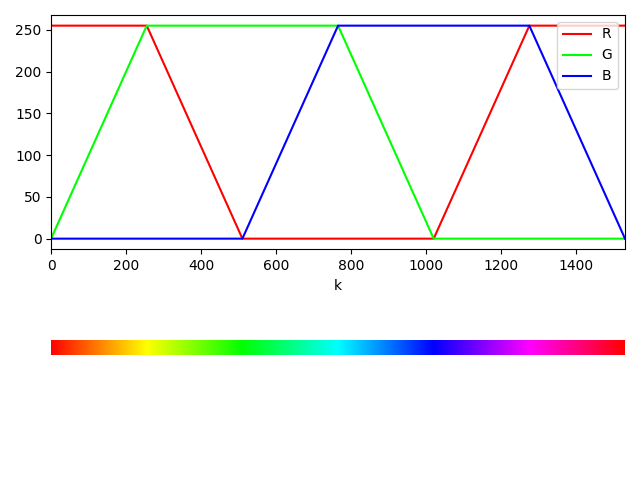
\includegraphics[width = \textwidth]{img/colors}
				\caption{Wartości składników RGB w kolejnych krokach działania algorytmu wraz z odpowiadającymi im kolorami.}
			\end{figure}
		\subsection{Generowanie odcinków krzywej w klasie CurveGenerator}
			\begin{lstlisting}
				Segment CurveGenerator::generate_segment()
				{
					Point start = m_curve.get_pos(m_t, m_is_cartesian);
					double current_segment_length = 0;
					Point pos;
					int i = 0;
					while (current_segment_length < m_segment_length && i < 400)
					{
						i++;
						pos = m_curve.get_pos(m_t += m_segment_generation_step, m_is_cartesian);
						current_segment_length = sqrt(pow(start.x - pos.x, 2) + pow(start.y - pos.y, 2) + pow(start.z - pos.z, 2));
					}
					return Segment(start, pos, color.next());
				}
			\end{lstlisting}
			Po ustaleniu położenie krzywej dla argumentu $t$, szukany jest odcinek o zadanej długości poprzez stopniowe zwiększanie parametru $t$.
			Poszukiwanie zostaje przerwane jeżeli zostanie znaleziony odcinek o pożądanej długości lub przekroczona zostanie maksymalna liczba iteracji (tu: 400).
		\subsection{Generowanie krzywej w klasie CurveGenerator}
			\begin{lstlisting}
				std::deque<Segment> CurveGenerator::get_next()
				{
					if (m_animate)
					{
						Segment seg = generate_segment();
				
						if (m_current_segment_count > m_max_animation_segment_count)
						{
							m_queue.pop_front();
						}
						else
							m_current_segment_count++;
				
						m_queue.push_back(seg);
				
						for (int i = 0; i < m_current_segment_count - 0.6 * m_max_animation_segment_count; i++)
							m_queue[i].color += (int)(255.0 / (0.4 * m_max_animation_segment_count));
				
						return m_queue;
					}
					else
					{
						while (m_current_segment_count < m_max_segment_count)
						{
							m_current_segment_count++;
							Segment seg = generate_segment();
							m_queue.push_back(seg);
						}
					}
					return m_queue;
				}
			\end{lstlisting}
			W zależności od tego czy krzywa ma być animowana czy nie, algorytm zachowuje się w różny sposób.
			W pierwszym przypadku kolejne segmenty dokładane są tak długo, aż nie zostanie osiągnięty ich limit. Wtedy w każdej iteracji poza dodaniem nowego segmentu jednocześnie usuwany jest najstarszy segment należący do krzywej.
			Jednocześnie, jeżeli długość krzywej zacznie przekraczać 60\% maksymalnej długości, najstarsze segmenty zostają stopniowo rozjaśniane.
			Jeżeli krzywa nie jest animowana, funkcja generuje po prostu całość krzywej na raz.
			
\section{Kodowanie}
Opis klas:
\begin{itemize}
	\item Vector4 – reprezentuje wektor o czterech składowych zawierająca położenie punktu (konstruktor ustawia automatycznie wartość czwartej składowej na 1),
	\item Matrix4 – reprezentuje macierz przekształcenia o wymiarach 4x4 (konstruktor ustawia automatycznie wartość elementu (4, 4) na 1),
	\item GUIMyFrame1 – odpowiedzialna za wszelkie metody zmieniające wartości parametrów i rysujące krzywą.
\end{itemize}

Opis metod:
\begin{itemize}
	\item	Vector4::Set – pozwala ustawić współrzędne wektora,
	\item 	Vector4::GetX – pobranie współrzędnej x,
	\item 	Vector4::GetY – pobranie współrzędnej y,
	\item 	Vector4::GetZ – pobranie współrzędnej z,
	\item 	Vector4::operator- - przeciążony operator odejmowania dla wektorów,
	\item 	operator* - przeciążone operatory * dla operacji Matrix4 * Matrix4, Matix4 * Vector4 oraz Vector4 * value,
	\item 	RotateX – obracanie wokół osi x,
	\item 	RotateY – obracanie wokół osi y,
	\item 	RotateZ – obracanie wokół osi z,
	\item 	Projection – dostosowywanie rysowanej krzywej do wymiarów panelu,
	\item 	Normalization – normalizacja wektora położenia punktu, tak by zawierał się w obszarze panelu,
	\item 	Repaint – funkcja rysująca krzywą na podstawie tablicy położeń punktów i macierzy przekształceń.
\end{itemize}

Opis zmiennych:
\begin{itemize}
\item	float m\_curve\_segment\_count – ilość segmentów, z których składa się krzywa,
\item	float m\_curve\_segment\_length – długość pojedynczego segmentu,
\item	bool m\_cartesian – przechowuje informację, czy krzywa ma być rysowana we współrzędnych kartezjańskich (jeśli prawda – tak, jeśli nieprawda- program rysuje we współrzędnych biegunowych),
\item	CurveGenerator m\_generator – generator segmentów krzywej,
\item 	Std::deque$<Segment>$ m\_data – tablica zawierająca położenia wszystkich segmentów krzywej,
\item	Vector4 m\_rotation – wektor rotacji.

\end{itemize}

\section{Testowanie}
Testowanie odbywało się w cotygodniowych odstępach czasu. Każdy z trzech programistów kompilował wspólnie złożony kod na swojej maszynie i szukał błędów w działaniu program. Znalezione błędy były spisywane, a następnie rozdzielane na poszczególnych developerów jako dodatkowe zadania do realizacji w następnym tygodniu. Gdy napotykano problemy, które sprawiały większe trudności zespół wspólnie analizował możliwe rozwiązania. Program był także pokazywany osobom kompletnie z nim nie związanymi z procesem jego tworzenia w celu zaczerpnięcia obiektywnej opinii  na temat aktualnej prezencji i możliwych udoskonaleniach.
\section{Wdrożenie, raport i wnioski}
\end{document}